\chapter{PK7 --- Khảo sát gu}
\clearpage\begin{landscape}
\begin{figure}[H]\centering
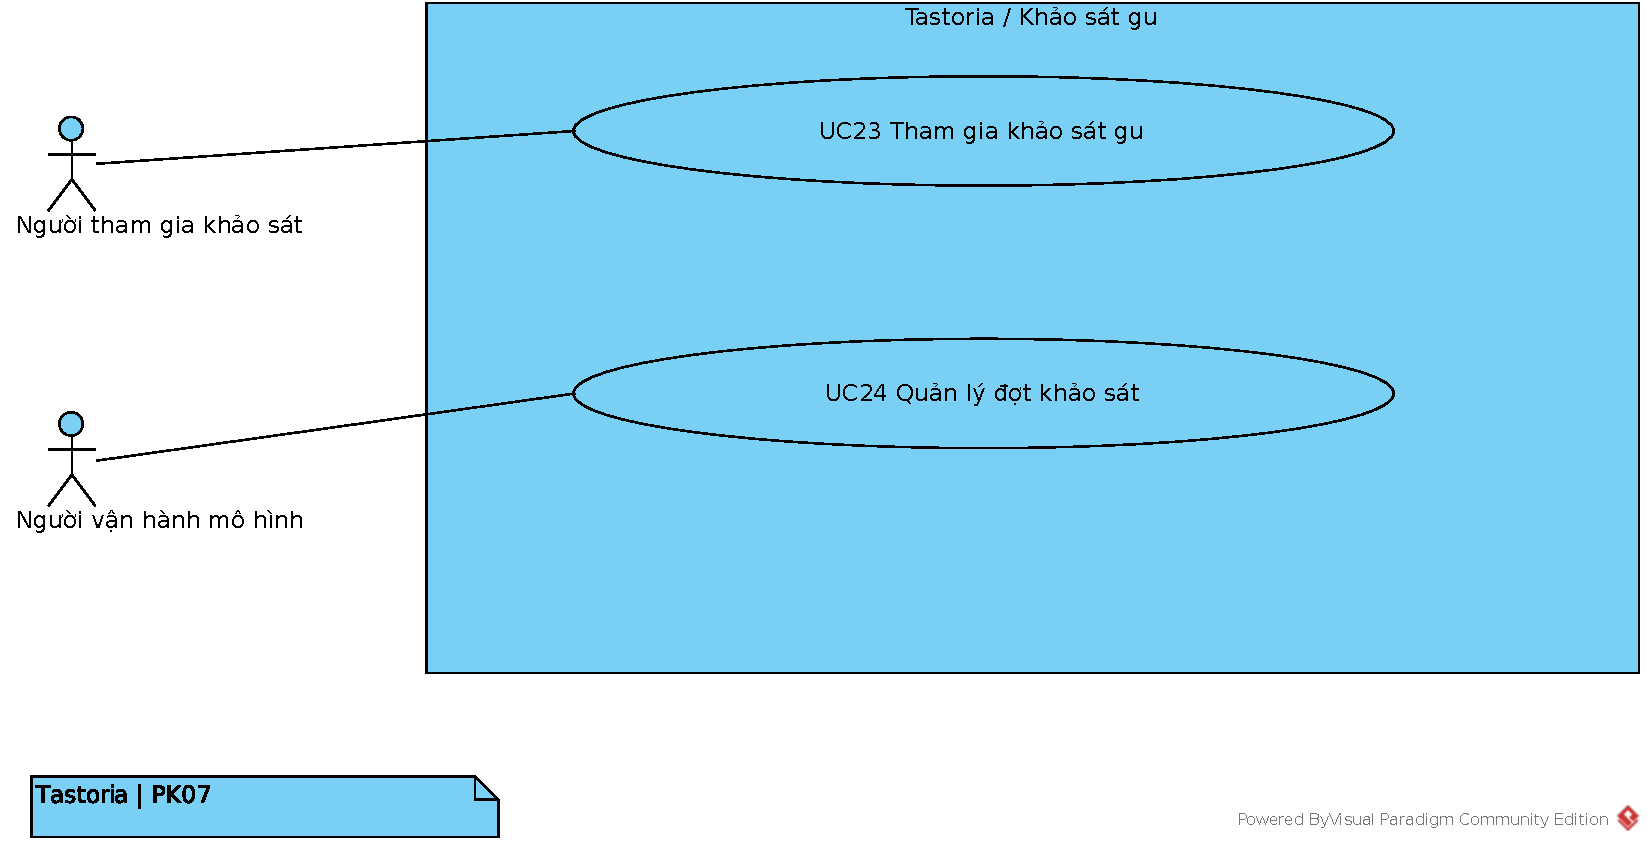
\includegraphics[width=0.96\linewidth,height=0.78\textwidth,keepaspectratio]{assets/PK07.pdf}
\caption{PK07 --- Phân rã use case}\label{fig:Phu-luc-A-Use-Cases:7}
\end{figure}
\end{landscape}\clearpage
\section{UC23 --- Tham gia khảo sát gu món ăn}
\subsection{Mục tiêu trong ngữ cảnh}
Một người ngoài (A03), không cần tài khoản, mở link hoặc quét mã QR của đợt khảo sát, đồng ý tham gia, chấm điểm 1--5 khoảng 45 món (10 món neo chung cho mọi người và khoảng 35 món rút ngẫu nhiên phân tầng theo loại món) hoặc chọn "chưa ăn bao giờ", rồi chọn tối đa 5 món hay ăn. Dữ liệu này là nguồn huấn luyện và đánh giá bộ xếp hạng gu. Phiếu không hỏi thông tin sức khoẻ hay định danh.

\subsection{Phạm vi và mức}
\begin{itemize}
\item Phạm vi: hệ thống Tastoria (trang khảo sát web + backend), hộp đen.
\item Mức: mục tiêu người dùng.
\end{itemize}
\subsection{Tác nhân và bên liên quan (quyền lợi)}
{\footnotesize\setlength{\tabcolsep}{0pt}
\begin{longtable}{@{}L{7.850cm}@{\hspace{3mm}}L{7.850cm}@{}}
\caption{Tác nhân và bên liên quan (quyền lợi)}\\
\toprule
\textbf{Bên} & \textbf{Quyền lợi} \\
\midrule\endfirsthead
\multicolumn{2}{l}{\small\itshape Bảng \thetable{} (tiếp theo)}\\
\toprule
\textbf{Bên} & \textbf{Quyền lợi} \\
\midrule\endhead
\bottomrule\endfoot
A03 Người tham gia khảo sát & Ẩn danh; biết rõ dữ liệu dùng làm gì trước khi đồng ý; làm dở rồi quay lại tiếp được; thao tác nhanh trên điện thoại. \\ \addlinespace[3pt]
A06 Người vận hành mô hình & Mỗi phiếu theo đúng thiết kế khối không đầy đủ của đợt (đủ món neo, phân tầng đúng), có bằng chứng đồng ý gắn phiên bản điều khoản. \\ \addlinespace[3pt]
Nhóm dự án & Không có dữ liệu bịa; phiếu bỏ dở phân biệt được với phiếu hoàn tất. \\ \addlinespace[3pt]
\end{longtable}}
\subsection{Tiền điều kiện}
\begin{enumerate}
\item Có đúng một {\small\texttt{survey\_\allowbreak{}\allowbreak{}forms}} đang mở ({\small\texttt{is\_\allowbreak{}\allowbreak{}open = true}}), tạo ở UC24.
\item Mục đích {\small\texttt{survey}} có một {\small\texttt{policy\_\allowbreak{}\allowbreak{}versions}} hiện hành ({\small\texttt{effective\_\allowbreak{}\allowbreak{}from \ensuremath{\leq} now()}}).
\end{enumerate}
\subsection{Đảm bảo tối thiểu}
\begin{itemize}
\item Không lưu gì về A03 trước khi A03 tự tích đồng ý {\small\texttt{survey}} (không tích sẵn).
\item Không lưu email, tên, số điện thoại, IP hay thông tin sức khoẻ của A03.
\item Mỗi điểm chỉ thuộc một cặp (người tham gia, món) đã được giao; gửi lại không tạo bản ghi trùng.
\end{itemize}
\subsection{Đảm bảo khi thành công}
\begin{itemize}
\item Có một {\small\texttt{survey\_\allowbreak{}\allowbreak{}respondents}} với {\small\texttt{policy\_\allowbreak{}\allowbreak{}version\_\allowbreak{}\allowbreak{}id}}, {\small\texttt{consented\_\allowbreak{}\allowbreak{}at}}, {\small\texttt{channel}}, {\small\texttt{completed\_\allowbreak{}\allowbreak{}at}}.
\item {\small\texttt{survey\_\allowbreak{}\allowbreak{}assignments}} có {\small\texttt{n\_\allowbreak{}\allowbreak{}anchor}} món neo ({\small\texttt{is\_\allowbreak{}\allowbreak{}anchor = true}}) và {\small\texttt{n\_\allowbreak{}\allowbreak{}random}} món ngẫu nhiên, thứ tự hiển thị trộn ngẫu nhiên.
\item Mỗi món được giao có đúng một {\small\texttt{survey\_\allowbreak{}\allowbreak{}ratings}} (điểm 1--5 hoặc {\small\texttt{never\_\allowbreak{}\allowbreak{}eaten = true}}).
\item {\small\texttt{survey\_\allowbreak{}\allowbreak{}favorites}} có tối đa 5 món.
\end{itemize}
\subsection{Kích hoạt}
A03 mở link khảo sát ({\small\texttt{channel = link}}) hoặc quét mã QR ({\small\texttt{channel = qr}}).

\subsection{Kịch bản chính}
\begin{enumerate}
\item A03 mở trang khảo sát; trang gọi {\small\texttt{GET /\allowbreak{}\allowbreak{}policies/\allowbreak{}\allowbreak{}\{purpose\}/\allowbreak{}\allowbreak{}current}} với {\small\texttt{purpose = survey}}.
\item Module {\small\texttt{privacy}} trả {\small\texttt{consent\_\allowbreak{}\allowbreak{}purposes}} (tên, mô tả, loại dữ liệu) và nội dung {\small\texttt{policy\_\allowbreak{}\allowbreak{}versions}} hiện hành.
\item Trang hiện mục đích, dữ liệu thu, thời gian lưu và ô "Tôi đồng ý" chưa tích (BR-\allowbreak{}CONSENT-\allowbreak{}01); A03 đọc và tự tích, chạm "Bắt đầu".
\item Trang gửi {\small\texttt{POST /\allowbreak{}\allowbreak{}survey/\allowbreak{}\allowbreak{}respondents}} với {\small\texttt{policy\_\allowbreak{}\allowbreak{}version\_\allowbreak{}\allowbreak{}id}}, {\small\texttt{channel}}, cờ đồng ý.
\item Module {\small\texttt{survey}} kiểm cờ đồng ý và {\small\texttt{policy\_\allowbreak{}\allowbreak{}version\_\allowbreak{}\allowbreak{}id}} hiện hành qua {\small\texttt{privacy}}, lấy form đang mở.
\item Module {\small\texttt{survey}} ghi {\small\texttt{survey\_\allowbreak{}\allowbreak{}respondents}}, rồi sinh {\small\texttt{survey\_\allowbreak{}\allowbreak{}assignments}}: toàn bộ món neo của form ({\small\texttt{survey\_\allowbreak{}\allowbreak{}form\_\allowbreak{}\allowbreak{}anchors}}) + {\small\texttt{n\_\allowbreak{}\allowbreak{}random}} món rút ngẫu nhiên không lặp từ các món {\small\texttt{published}} không phải neo, phân tầng theo {\small\texttt{slot}} (man, rau, canh) tỷ lệ với số món mỗi slot trong kho (gọi {\small\texttt{catalog}} lấy danh sách món); trộn {\small\texttt{display\_\allowbreak{}\allowbreak{}order}} ngẫu nhiên.
\item Hệ thống trả {\small\texttt{201}} kèm {\small\texttt{respondent\_\allowbreak{}\allowbreak{}id}} và {\small\texttt{respondent\_\allowbreak{}\allowbreak{}token}} (token ký, chỉ mở được phiếu này); trang lưu cả hai trên trình duyệt.
\item Trang gọi {\small\texttt{GET /\allowbreak{}\allowbreak{}survey/\allowbreak{}\allowbreak{}respondents/\allowbreak{}\allowbreak{}\{id\}}} (kèm token) lấy danh sách món theo {\small\texttt{display\_\allowbreak{}\allowbreak{}order}}, tên và ảnh minh hoạ món, câu đã trả lời.
\item Với mỗi món, A03 chọn một điểm 1--5 hoặc "Chưa ăn bao giờ"; trang gửi {\small\texttt{PUT /\allowbreak{}\allowbreak{}survey/\allowbreak{}\allowbreak{}respondents/\allowbreak{}\allowbreak{}\{id\}/\allowbreak{}\allowbreak{}ratings/\allowbreak{}\allowbreak{}\{recipeId\}}}.
\item Module {\small\texttt{survey}} kiểm món thuộc {\small\texttt{survey\_\allowbreak{}\allowbreak{}assignments}} của người này, ghi đè hoặc tạo {\small\texttt{survey\_\allowbreak{}\allowbreak{}ratings}} ({\small\texttt{rating}} NULL khi {\small\texttt{never\_\allowbreak{}\allowbreak{}eaten = true}}), cập nhật {\small\texttt{answered\_\allowbreak{}\allowbreak{}at}}. Bước 9--10 lặp tới hết danh sách.
\item Trang hiện câu "Chọn tối đa 5 món bạn hay ăn" với ô tìm món; A03 chọn và chạm "Lưu"; trang gửi {\small\texttt{PUT /\allowbreak{}\allowbreak{}survey/\allowbreak{}\allowbreak{}respondents/\allowbreak{}\allowbreak{}\{id\}/\allowbreak{}\allowbreak{}favorites}}.
\item Module {\small\texttt{survey}} thay toàn bộ {\small\texttt{survey\_\allowbreak{}\allowbreak{}favorites}} của người này bằng danh sách mới.
\item A03 chạm "Gửi phiếu"; trang gửi {\small\texttt{POST /\allowbreak{}\allowbreak{}survey/\allowbreak{}\allowbreak{}respondents/\allowbreak{}\allowbreak{}\{id\}/\allowbreak{}\allowbreak{}complete}}.
\item Module {\small\texttt{survey}} kiểm mọi món được giao đã có trả lời, đặt {\small\texttt{completed\_\allowbreak{}\allowbreak{}at}}.
\item Hệ thống trả {\small\texttt{200}}; trang hiện lời cảm ơn và xoá token khỏi trình duyệt.
\end{enumerate}
\subsection{Mở rộng}
\begin{itemize}
\item \textbf{1a. Không có form đang mở:} {\small\texttt{POST /\allowbreak{}\allowbreak{}survey/\allowbreak{}\allowbreak{}respondents}} trả {\small\texttt{409}}, {\small\texttt{code = survey\_\allowbreak{}\allowbreak{}closed}}; trang hiện "Đợt khảo sát đã đóng".
\item \textbf{3a. A03 không tích đồng ý:} nút "Bắt đầu" bị khoá; không gửi yêu cầu nào; không lưu gì.
\item \textbf{4a. Yêu cầu tới server mà cờ đồng ý false hoặc thiếu:} trả {\small\texttt{422}}, {\small\texttt{code = consent\_\allowbreak{}\allowbreak{}required}}; không ghi bảng nào.
\item \textbf{4b. {\small\texttt{policy\_\allowbreak{}\allowbreak{}version\_\allowbreak{}\allowbreak{}id}} không phải bản hiện hành (trang mở từ trước khi điều khoản đổi):} trả {\small\texttt{409}}, {\small\texttt{code = policy\_\allowbreak{}\allowbreak{}outdated}}; trang tải lại điều khoản và yêu cầu đồng ý lại.
\item \textbf{4c. Mất mạng khi gửi {\small\texttt{POST /\allowbreak{}\allowbreak{}survey/\allowbreak{}\allowbreak{}respondents}} (không lũy đẳng):} trang gửi lại; nếu lần đầu đã tới server thì sinh ra một người tham gia rỗng thứ hai. Phiếu rỗng không có {\small\texttt{completed\_\allowbreak{}\allowbreak{}at}} nên bị loại khi xuất (UC24).
\item \textbf{6a. Kho món {\small\texttt{published}} ít hơn {\small\texttt{n\_\allowbreak{}\allowbreak{}random}} món ngoài neo:} trả {\small\texttt{503}}, {\small\texttt{code = survey\_\allowbreak{}\allowbreak{}form\_\allowbreak{}\allowbreak{}misconfigured}} và ghi log để A06 xử lý ở UC24; rollback, không tạo người tham gia.
\item \textbf{8a. A03 đóng trang rồi quay lại:} trang dùng {\small\texttt{respondent\_\allowbreak{}\allowbreak{}id}} và token đã lưu, gọi {\small\texttt{GET /\allowbreak{}\allowbreak{}survey/\allowbreak{}\allowbreak{}respondents/\allowbreak{}\allowbreak{}\{id\}}} và tiếp tục ở món chưa trả lời đầu tiên.
\item \textbf{8b. Token sai, hết hạn hoặc thuộc người tham gia khác:} trả {\small\texttt{401}}; trang mời bắt đầu phiếu mới.
\item \textbf{8c. Form bị đóng khi A03 đang làm:} các lệnh ghi trả {\small\texttt{409}} {\small\texttt{survey\_\allowbreak{}\allowbreak{}closed}}; phần đã trả lời giữ nguyên; trang thông báo đợt đã đóng.
\item \textbf{9a. Mất mạng khi chấm:} trang giữ hàng đợi các lệnh {\small\texttt{PUT}} và gửi lại khi có mạng; {\small\texttt{PUT}} lũy đẳng nên gửi nhiều lần cho kết quả như một lần.
\item \textbf{9b. A03 đổi ý điểm một món đã chấm:} gửi {\small\texttt{PUT}} mới, ghi đè giá trị cũ.
\item \textbf{10a. Điểm ngoài 1--5, hoặc có điểm đồng thời {\small\texttt{never\_\allowbreak{}\allowbreak{}eaten = true}}:} trả {\small\texttt{422}}, {\small\texttt{code = invalid\_\allowbreak{}\allowbreak{}rating}}; không ghi.
\item \textbf{10b. {\small\texttt{recipeId}} không nằm trong danh sách được giao:} trả {\small\texttt{404}}; không ghi.
\item \textbf{11a. Chọn quá 5 món, món trùng hoặc món không {\small\texttt{published}}:} trả {\small\texttt{422}}, {\small\texttt{code = invalid\_\allowbreak{}\allowbreak{}favorites}}; không thay đổi danh sách cũ.
\item \textbf{11b. A03 bỏ qua câu món hay ăn:} cho phép; {\small\texttt{survey\_\allowbreak{}\allowbreak{}favorites}} rỗng.
\item \textbf{14a. Còn món chưa trả lời:} trả {\small\texttt{422}}, {\small\texttt{code = survey\_\allowbreak{}\allowbreak{}incomplete}} kèm danh sách {\small\texttt{recipeId}} còn thiếu; trang cuộn tới món đầu tiên còn thiếu.
\item \textbf{14b. Gửi "Gửi phiếu" lần nữa khi đã hoàn tất:} trả {\small\texttt{200}} với {\small\texttt{completed\_\allowbreak{}\allowbreak{}at}} cũ, không đổi.
\item \textbf{14c. Ghi sau khi đã hoàn tất:} các lệnh {\small\texttt{PUT}} trả {\small\texttt{409}}, {\small\texttt{code = survey\_\allowbreak{}\allowbreak{}already\_\allowbreak{}\allowbreak{}completed}}.
\item \textbf{Mọi bước: lỗi hệ thống:} trả {\small\texttt{503}} {\small\texttt{application/\allowbreak{}\allowbreak{}problem+json}}; trang hiện "Chưa lưu được, thử lại" và giữ hàng đợi.
\end{itemize}
\subsection{Ghi chú đối chiếu của báo cáo}
Giữ phạm vi yêu cầu của đặc tả nguồn; cần kiểm thử theo môi trường và phiên bản thực tế trước khi ghi kết quả nghiệm thu.

\textbf{Nguồn:} {\small\texttt{Tastoria/\allowbreak{}\allowbreak{}docs/\allowbreak{}\allowbreak{}sad/\allowbreak{}\allowbreak{}use-\allowbreak{}cases/\allowbreak{}\allowbreak{}UC23.\allowbreak{}md}}. Mã nghiệp vụ: BR-\allowbreak{}CONSENT-\allowbreak{}01, BR-\allowbreak{}CATALOG-\allowbreak{}01.

\textbf{Dữ liệu liên quan:} {\small\texttt{consent\_\allowbreak{}\allowbreak{}purposes}}, {\small\texttt{policy\_\allowbreak{}\allowbreak{}versions}}, {\small\texttt{survey\_\allowbreak{}\allowbreak{}forms}}, {\small\texttt{survey\_\allowbreak{}\allowbreak{}form\_\allowbreak{}\allowbreak{}anchors}}, {\small\texttt{recipes}}, {\small\texttt{survey\_\allowbreak{}\allowbreak{}respondents}}, {\small\texttt{survey\_\allowbreak{}\allowbreak{}assignments}}, {\small\texttt{survey\_\allowbreak{}\allowbreak{}ratings}}, {\small\texttt{survey\_\allowbreak{}\allowbreak{}favorites}}.

\textbf{Điểm giao tiếp:} {\small\texttt{GET /\allowbreak{}\allowbreak{}policies/\allowbreak{}\allowbreak{}\{purpose\}/\allowbreak{}\allowbreak{}current}}; {\small\texttt{POST /\allowbreak{}\allowbreak{}survey/\allowbreak{}\allowbreak{}respondents}}; {\small\texttt{GET /\allowbreak{}\allowbreak{}survey/\allowbreak{}\allowbreak{}respondents/\allowbreak{}\allowbreak{}\{id\}}}; {\small\texttt{PUT /\allowbreak{}\allowbreak{}survey/\allowbreak{}\allowbreak{}respondents/\allowbreak{}\allowbreak{}\{id\}/\allowbreak{}\allowbreak{}ratings/\allowbreak{}\allowbreak{}\{recipeId\}}}; {\small\texttt{PUT /\allowbreak{}\allowbreak{}survey/\allowbreak{}\allowbreak{}respondents/\allowbreak{}\allowbreak{}\{id\}/\allowbreak{}\allowbreak{}favorites}}; {\small\texttt{POST /\allowbreak{}\allowbreak{}survey/\allowbreak{}\allowbreak{}respondents/\allowbreak{}\allowbreak{}\{id\}/\allowbreak{}\allowbreak{}complete}}.

\section{UC24 --- Quản lý đợt khảo sát (tạo phiếu, xuất kết quả)}
\subsection{Mục tiêu trong ngữ cảnh}
Người vận hành mô hình (A06) mở một đợt khảo sát gu theo thiết kế khối không đầy đủ (mặc định 10 món neo + 35 món ngẫu nhiên phân tầng), theo dõi số người tham gia, và cuối đợt xuất kết quả ra tệp để huấn luyện và đánh giá bộ xếp hạng gu. Mọi thao tác chạy bằng CLI trong container {\small\texttt{api}}, có ghi nhật ký kiểm toán.

\subsection{Phạm vi và mức}
\begin{itemize}
\item Phạm vi: hệ thống Tastoria (CLI nhân sự + endpoint quản trị), hộp đen.
\item Mức: mục tiêu người dùng.
\end{itemize}
\subsection{Tác nhân và bên liên quan (quyền lợi)}
{\footnotesize\setlength{\tabcolsep}{0pt}
\begin{longtable}{@{}L{7.850cm}@{\hspace{3mm}}L{7.850cm}@{}}
\caption{Tác nhân và bên liên quan (quyền lợi)}\\
\toprule
\textbf{Bên} & \textbf{Quyền lợi} \\
\midrule\endfirsthead
\multicolumn{2}{l}{\small\itshape Bảng \thetable{} (tiếp theo)}\\
\toprule
\textbf{Bên} & \textbf{Quyền lợi} \\
\midrule\endhead
\bottomrule\endfoot
A06 Người vận hành mô hình & Tạo form tái lập được (danh sách neo cố định, ghi lại); xuất dữ liệu sạch, đủ cột để phân tích; biết tiến độ đợt. \\ \addlinespace[3pt]
A03 Người tham gia khảo sát & Dữ liệu xuất ra không có định danh; chỉ gồm người đã đồng ý. \\ \addlinespace[3pt]
Người chấm (giảng viên) & Thiết kế phiếu và tệp xuất truy được về phiên bản form, phiên bản kho món và phiên bản điều khoản. \\ \addlinespace[3pt]
\end{longtable}}
\subsection{Tiền điều kiện}
\begin{enumerate}
\item A06 có tài khoản {\small\texttt{users.\allowbreak{}role = ml\_\allowbreak{}\allowbreak{}operator}} và quyền chạy lệnh trong container {\small\texttt{api}}.
\item Kho món có ít nhất {\small\texttt{N + M}} món {\small\texttt{published}} (đã nhập ở UC25), mỗi slot {\small\texttt{man}}, {\small\texttt{rau}}, {\small\texttt{canh}} đều có món.
\end{enumerate}
\subsection{Đảm bảo tối thiểu}
\begin{itemize}
\item Tại mọi thời điểm có nhiều nhất một form {\small\texttt{is\_\allowbreak{}\allowbreak{}open = true}}.
\item Form đã có người tham gia không bị sửa danh sách neo hay {\small\texttt{n\_\allowbreak{}\allowbreak{}anchor}}, {\small\texttt{n\_\allowbreak{}\allowbreak{}random}}.
\item Mọi lần chạy lệnh (thành công hoặc lỗi nghiệp vụ) có một dòng {\small\texttt{audit\_\allowbreak{}\allowbreak{}log}}.
\end{itemize}
\subsection{Đảm bảo khi thành công}
\begin{itemize}
\item Tạo form: có một {\small\texttt{survey\_\allowbreak{}\allowbreak{}forms}} mới với {\small\texttt{version}} duy nhất, {\small\texttt{n\_\allowbreak{}\allowbreak{}anchor = N}}, {\small\texttt{n\_\allowbreak{}\allowbreak{}random = M}}, {\small\texttt{is\_\allowbreak{}\allowbreak{}open = true}}; đúng N dòng {\small\texttt{survey\_\allowbreak{}\allowbreak{}form\_\allowbreak{}\allowbreak{}anchors}}; form mở trước đó (nếu có) chuyển {\small\texttt{is\_\allowbreak{}\allowbreak{}open = false}}.
\item Xuất: có các tệp CSV UTF-\allowbreak{}8 của form trong thư mục xuất, kèm tệp mô tả (manifest) ghi phiên bản form, số người, sha256 từng tệp.
\end{itemize}
\subsection{Kích hoạt}
A06 chạy {\small\texttt{tastoria survey create-\allowbreak{}form -\allowbreak{}-\allowbreak{}anchors N -\allowbreak{}-\allowbreak{}random M}} để mở đợt, hoặc {\small\texttt{tastoria survey export <form\_\allowbreak{}\allowbreak{}version>}} để xuất kết quả; A06 mở danh sách đợt ({\small\texttt{GET /\allowbreak{}\allowbreak{}admin/\allowbreak{}\allowbreak{}surveys}}) để theo dõi.

\subsection{Kịch bản chính}
\textbf{Luồng A --- tạo form và mở đợt}

\begin{enumerate}
\item A06 chạy {\small\texttt{tastoria survey create-\allowbreak{}form -\allowbreak{}-\allowbreak{}anchors 10 -\allowbreak{}-\allowbreak{}random 35}}.
\item Module {\small\texttt{admin}} xác thực A06 với vai trò {\small\texttt{ml\_\allowbreak{}\allowbreak{}operator}} qua {\small\texttt{identity}}.
\item Module {\small\texttt{admin}} gọi {\small\texttt{catalog}} lấy các món {\small\texttt{published}} theo slot, kiểm N \ensuremath{\geq} 1, M \ensuremath{\geq} 1, N + M \ensuremath{\leq} số món {\small\texttt{published}}.
\item Module {\small\texttt{admin}} gọi {\small\texttt{survey.\allowbreak{}create\_\allowbreak{}\allowbreak{}form(N, M)}}: module {\small\texttt{survey}} rút N món neo phân tầng theo slot (tỷ lệ với số món mỗi slot, hạt giống ngẫu nhiên được in ra và ghi vào {\small\texttt{audit\_\allowbreak{}\allowbreak{}log}}), sinh {\small\texttt{version}} mới.
\item Trong một giao dịch, module {\small\texttt{survey}} đóng form đang mở ({\small\texttt{is\_\allowbreak{}\allowbreak{}open = false}}), ghi {\small\texttt{survey\_\allowbreak{}\allowbreak{}forms}} mới ({\small\texttt{is\_\allowbreak{}\allowbreak{}open = true}}) và {\small\texttt{survey\_\allowbreak{}\allowbreak{}form\_\allowbreak{}\allowbreak{}anchors}}.
\item Module {\small\texttt{admin}} gọi {\small\texttt{privacy}} ghi {\small\texttt{audit\_\allowbreak{}\allowbreak{}log}} ({\small\texttt{actor\_\allowbreak{}\allowbreak{}role = ml\_\allowbreak{}\allowbreak{}operator}}, {\small\texttt{action = survey.\allowbreak{}create\_\allowbreak{}\allowbreak{}form}}, {\small\texttt{entity = survey\_\allowbreak{}\allowbreak{}forms}}, {\small\texttt{entity\_\allowbreak{}\allowbreak{}id}} = id form).
\item CLI in {\small\texttt{version}}, danh sách món neo theo slot, hạt giống, rồi thoát mã 0. Từ lúc này UC23 dùng form mới.
\end{enumerate}
\textbf{Luồng B --- theo dõi đợt}

\begin{enumerate}
\item A06 gọi {\small\texttt{GET /\allowbreak{}\allowbreak{}admin/\allowbreak{}\allowbreak{}surveys}} (vai trò {\small\texttt{ml\_\allowbreak{}\allowbreak{}operator}}).
\item Module {\small\texttt{admin}} gọi {\small\texttt{survey}} trả danh sách form: {\small\texttt{version}}, {\small\texttt{is\_\allowbreak{}\allowbreak{}open}}, {\small\texttt{n\_\allowbreak{}\allowbreak{}anchor}}, {\small\texttt{n\_\allowbreak{}\allowbreak{}random}}, {\small\texttt{created\_\allowbreak{}\allowbreak{}at}}, số người tham gia, số người hoàn tất, số điểm trung bình mỗi món (không neo).
\end{enumerate}
\textbf{Luồng C --- xuất kết quả}

\begin{enumerate}
\item A06 chạy {\small\texttt{tastoria survey export <form\_\allowbreak{}\allowbreak{}version>}}.
\item Module {\small\texttt{admin}} xác thực vai trò, gọi {\small\texttt{survey.\allowbreak{}export(form\_\allowbreak{}\allowbreak{}version)}}.
\item Module {\small\texttt{survey}} đọc người tham gia có {\small\texttt{completed\_\allowbreak{}\allowbreak{}at}} khác NULL của form và ghi các tệp: {\small\texttt{respondents.\allowbreak{}csv}} ({\small\texttt{respondent\_\allowbreak{}\allowbreak{}id}}, {\small\texttt{policy\_\allowbreak{}\allowbreak{}version}}, {\small\texttt{consented\_\allowbreak{}\allowbreak{}at}}, {\small\texttt{completed\_\allowbreak{}\allowbreak{}at}}, {\small\texttt{channel}}), {\small\texttt{assignments.\allowbreak{}csv}} ({\small\texttt{respondent\_\allowbreak{}\allowbreak{}id}}, {\small\texttt{recipe\_\allowbreak{}\allowbreak{}id}}, {\small\texttt{display\_\allowbreak{}\allowbreak{}order}}, {\small\texttt{is\_\allowbreak{}\allowbreak{}anchor}}), {\small\texttt{ratings.\allowbreak{}csv}} ({\small\texttt{respondent\_\allowbreak{}\allowbreak{}id}}, {\small\texttt{recipe\_\allowbreak{}\allowbreak{}id}}, {\small\texttt{rating}}, {\small\texttt{never\_\allowbreak{}\allowbreak{}eaten}}, {\small\texttt{answered\_\allowbreak{}\allowbreak{}at}}), {\small\texttt{favorites.\allowbreak{}csv}}, {\small\texttt{anchors.\allowbreak{}csv}}, {\small\texttt{recipes.\allowbreak{}csv}} ({\small\texttt{recipe\_\allowbreak{}\allowbreak{}id}}, {\small\texttt{name\_\allowbreak{}\allowbreak{}vi}}, {\small\texttt{slot}}, {\small\texttt{status}}), và {\small\texttt{manifest.\allowbreak{}json}}.
\item Module {\small\texttt{admin}} ghi {\small\texttt{audit\_\allowbreak{}\allowbreak{}log}} ({\small\texttt{action = survey.\allowbreak{}export}}, {\small\texttt{entity\_\allowbreak{}\allowbreak{}id}} = {\small\texttt{form\_\allowbreak{}\allowbreak{}version}}).
\item CLI in đường dẫn thư mục xuất, số người, số điểm, sha256 từng tệp; thoát mã 0.
\end{enumerate}
\subsection{Mở rộng}
\begin{itemize}
\item \textbf{1a. Thiếu hoặc sai tham số (N, M không phải số nguyên dương):} CLI in cách dùng, thoát mã 2; không ghi gì ngoài {\small\texttt{audit\_\allowbreak{}\allowbreak{}log}} lỗi.
\item \textbf{2a. Người chạy không có vai trò {\small\texttt{ml\_\allowbreak{}\allowbreak{}operator}}:} từ chối, thoát mã 1, ghi {\small\texttt{audit\_\allowbreak{}\allowbreak{}log}} với {\small\texttt{action = survey.\allowbreak{}denied}}. Với {\small\texttt{GET /\allowbreak{}\allowbreak{}admin/\allowbreak{}\allowbreak{}surveys}} trả {\small\texttt{403}}.
\item \textbf{3a. N + M lớn hơn số món {\small\texttt{published}}, hoặc có slot không có món nào:} thoát mã 1 với thông báo số món hiện có theo slot; không tạo form (không khả thi).
\item \textbf{4a. A06 muốn tái lập đúng danh sách neo:} đọc hạt giống trong {\small\texttt{audit\_\allowbreak{}\allowbreak{}log}} của lần tạo trước; lệnh hiện tại không nhận hạt giống làm tham số (xem câu hỏi mở 1).
\item \textbf{5a. Lỗi cơ sở dữ liệu giữa chừng:} rollback, form cũ vẫn mở, thoát mã 1. Chạy lại lệnh an toàn vì chưa có gì được ghi.
\item \textbf{5b. Chạy {\small\texttt{create-\allowbreak{}form}} hai lần liên tiếp:} lần hai tạo form thứ hai và đóng form thứ nhất; người đang làm phiếu form thứ nhất nhận {\small\texttt{409}} {\small\texttt{survey\_\allowbreak{}\allowbreak{}closed}} ở UC23. CLI hỏi xác nhận khi form đang mở đã có người tham gia.
\item \textbf{10a. {\small\texttt{form\_\allowbreak{}\allowbreak{}version}} không tồn tại:} thoát mã 1, in danh sách {\small\texttt{version}} hiện có.
\item \textbf{10b. Form đang mở:} vẫn xuất (ảnh chụp tại thời điểm chạy), {\small\texttt{manifest.\allowbreak{}json}} ghi {\small\texttt{is\_\allowbreak{}\allowbreak{}open = true}} và thời điểm xuất; CLI in cảnh báo.
\item \textbf{10c. Chưa có người hoàn tất:} xuất tệp chỉ có tiêu đề cột, {\small\texttt{manifest.\allowbreak{}json}} ghi 0 người; thoát mã 0.
\item \textbf{12a. Món trong form đã chuyển {\small\texttt{retired}} (BR-\allowbreak{}CATALOG-\allowbreak{}01):} vẫn xuất theo đúng {\small\texttt{recipe\_\allowbreak{}\allowbreak{}id}} đã giao; {\small\texttt{recipes.\allowbreak{}csv}} ghi {\small\texttt{status = retired}}.
\item \textbf{12b. Thư mục xuất đã có tệp của lần xuất trước:} lệnh ghi vào thư mục mới có dấu thời gian, không ghi đè.
\item \textbf{12c. Hết dung lượng ổ khi ghi tệp:} xoá tệp dở, thoát mã 1.
\end{itemize}
\subsection{Ghi chú đối chiếu của báo cáo}
Giữ phạm vi yêu cầu của đặc tả nguồn; cần kiểm thử theo môi trường và phiên bản thực tế trước khi ghi kết quả nghiệm thu.

\textbf{Nguồn:} {\small\texttt{Tastoria/\allowbreak{}\allowbreak{}docs/\allowbreak{}\allowbreak{}sad/\allowbreak{}\allowbreak{}use-\allowbreak{}cases/\allowbreak{}\allowbreak{}UC24.\allowbreak{}md}}. Mã nghiệp vụ: BR-\allowbreak{}CATALOG-\allowbreak{}01, BR-\allowbreak{}CONSENT-\allowbreak{}01.

\textbf{Dữ liệu liên quan:} {\small\texttt{recipes}}, {\small\texttt{survey\_\allowbreak{}\allowbreak{}forms}}, {\small\texttt{survey\_\allowbreak{}\allowbreak{}form\_\allowbreak{}\allowbreak{}anchors}}, {\small\texttt{survey\_\allowbreak{}\allowbreak{}respondents}}, {\small\texttt{survey\_\allowbreak{}\allowbreak{}assignments}}, {\small\texttt{survey\_\allowbreak{}\allowbreak{}ratings}}, {\small\texttt{survey\_\allowbreak{}\allowbreak{}favorites}}, {\small\texttt{policy\_\allowbreak{}\allowbreak{}versions}}, {\small\texttt{audit\_\allowbreak{}\allowbreak{}log}}.

\textbf{Điểm giao tiếp:} {\small\texttt{CLI tastoria survey create-\allowbreak{}form -\allowbreak{}-\allowbreak{}anchors N -\allowbreak{}-\allowbreak{}random M}}; {\small\texttt{CLI tastoria survey export <form\_\allowbreak{}\allowbreak{}version>}}; {\small\texttt{GET /\allowbreak{}\allowbreak{}admin/\allowbreak{}\allowbreak{}surveys}}.
